% id: 0220
% book: RPM 중3-2 수학 · 02 삼각비의 활용
% section: 유형 13 실생활에서 직각삼각형의 변의 길이의 활용
% figure: crop:fig-0220.png
% answer: $2\sqrt{31}\mkern3mu \mathrm{km}$
% answer_source: 답지
% variant_level: 0 (원본 전사)
% 이 파일은 build.mjs 가 items.json 에서 만든다. 고칠 때는 items.json 을 고친다.
\noindent\begin{minipage}[t]{0.58\linewidth}\vspace{0pt}\raggedright 오른쪽 그림과 같이 두 척의 배가 $\pt{O}$~지점에서 동시에 출발하여 서로 다른 방향으로 시속 $5\mkern3mu \mathrm{km}$, $6\mkern3mu \mathrm{km}$로 이동하여 $2$시간 후 두 지점~$\pt{P}$, $\pt{Q}$에 각각 이르렀다. $\angle\pt{PON}=40^\circ$, $\angle\pt{QON}=20^\circ$일 때, 두 배 사이의 거리를 구하시오. \dmcondfill{배의 크기는 무시한다.}{}\end{minipage}\hfill\begin{minipage}[t]{0.4\linewidth}\vspace{0pt}\centering \setlength{\dmfigw}{69.3pt}\ifdim\dmfigw>\linewidth\setlength{\dmfigw}{\linewidth}\fi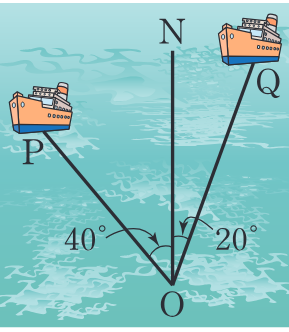
\includegraphics[width=\dmfigw]{figures/fig-0220.png}\end{minipage}\par
